%\documentclass[tikz]{beamer}
\documentclass[notheorems]{beamer}

%\usepackage{tikz}
%\usetikzlibrary{shapes,arrows}
\mode<presentation>{}
%\usepackage{beamerthemeshadow}
%\let\definition\relax
\let\theorem\relax
\input{../../paperProduction/occBind/docs/AMArepresentationNewCmds}


\author{Gary S. Anderson\thanks{The analysis and conclusions set forth are those of the author and do not indicate concurrence by other members of the research staff or the Board of Governors.}}

\title{A New Series Representation for 
Nonlinear Dynamic Stochastic Model Solutions:  Error Bounds and a New Solution Algorithm}

\date{\today: \currenttime}
\begin{document}


\begin{frame}
\maketitle
\end{frame}

\section{Introduction and Summary}

\begin{frame}
  \frametitle{Outline}
  \begin{itemize}
  \item Introduction
  \item Summary of Results
  \item The Series Representation
  \item Model Error Bounds
  \item A New Solution Algorithm
  \end{itemize}
\end{frame}

\subsection{Introduction}
  \frametitle{Introduction}
\label{sec:introduction0}
\begin{frame}
  \frametitle{Introduction}
  \begin{itemize}
  \item Novel representation for {\bf Bounded Time Invariant Maps}
  \item This {\bf Series Representation} plays and essential role in an algorithm for solving {\bf nonlinear} models with {\bf occasionally binding constraints} and/or {\bf regime switching}
  \item A {\bf robust} way to implement something similar to {\bf parameterized expectations}
  \end{itemize}
\end{frame}

\begin{frame}
  \frametitle{Introduction}
{\small
\begin{itemize}
\item Solutions characterized by: $\eqnFuncSys$  where, each 
\begin{gather}
\eqnFuncSysI{i}\equiv \eqnFuncSysIExpl{i} \label{eqnGates}
\end{gather}
\item Boolean valued gates, $\preGate_i\allArgs$ $\postGate_i\allArgs$,
$\lastGate_i\allArgs$. 
\item Model equations, $\eqnFunc_i$,  
\item ``Auxiliary variables'' as necessary
\item Exhaustive and mutually exclusive determining the solution  $x_t\tArg$
\item Employs a global projection method
\item Stochastic system leads to a deterministic and parallelizable equation systems
\end{itemize}
}
\end{frame}

\subsection{Summary of Results}
\label{sec:summary-results}




\begin{frame}
  \frametitle{Model Error Bounds}
  \begin{itemize}
  \item Exact (typically unknown) solution $x^\star_t=g^\star(x_{t-1},\epsilon_t)$ 
  \item Proposed solution  $x^p_t=g^p(x_{t-1},\epsilon_t), \,\,G^p(x)\equiv \expct{g^p(x_{t-1},\epsilon_t)}$ 
 \item Euler errors $\eulerE_i\tArg \equiv  \eqnFunc(x_{t-1},g^p(x_{t-1},\epsilon),G^p(g^p(x_{t-1},\epsilon)),\epsilon)$
 \item We can easily compute matrices  $F, \phi $ such that 
 {\small   \begin{gather*}
 \someNorm{ x^\star_{t}(x_{t-1},\epsilon) -	 x^p_{t}(x_{t-1},\epsilon)} \le 
 \max_{\{i,x_{t-1},\epsilon\}} \someNorm{(I-F)^{-1} \phi \eulerE_i\tArg }
    \end{gather*}}
  \end{itemize}
\end{frame}
\begin{frame}
  \frametitle{Some Related Work on Error Bounds}
  \begin{itemize}
  \item \cite{peralta-alva14} Error Upper Bound
    \begin{itemize}
\item Provide an empirical method for estimating the accuracy based on Euler equation errors when approximating continuous Markov equilibria
    \item Describe a robust algorithm for computing solutions and assessing accuracy in non optimal economies.\cite{feng14:_num}
    \end{itemize}
  \item \cite{judd2017lower} Error Lower Bound
    \begin{itemize}
    \item Forward Error Analysis but ``Allowing Euler equation, errors how small can approximation error be''
    \end{itemize}
  \end{itemize}
\end{frame}




\begin{frame}
  \frametitle{A New Algorithm}
 {\small  
\begin{itemize}
\item Using a formula from \citep{anderson10},
 \item Any bounded time invariant discrete map can be written as
    \begin{gather*}
      	 x\tArg =B x_{t-1}+ \phi \psi_\epsilon\epsilon + (I - F)^{-1} \phi \psi_c + \sum_{\sForSum=0}^\infty F^\sForSum \phi \ZWOarg(\expct{x_{t+\nu}})\\ \intertext{ so that}
\expct{ x_{t+1}\tArg} =B x\tArg  + (I - F)^{-1} \phi \psi_c+ \sum_{\sForSum =1}^\infty F^{\sForSum-1} \phi \ZWOarg(\expct{x_{t+\nu}}) 
    \end{gather*}
   \item If these functions satisfy the model equations you have a solution
   \item If not, use the $\eulerE_i \text{ and } \eqnFuncSys $ information to improve the solution
  \end{itemize}
}
\end{frame}

\begin{frame}
  \frametitle{Some Related Work on Solution Algorithms}
  \begin{itemize}
\item Similar in spirit to Parameterized Expectations\cite{haan90:_solvin_stoch}
\item Some work on efficient solution of regime switching models includes 
\cite{RePEc:bny:wpaper:0058}
\item Both \cite{holden15:_exist_dsge} and  \cite{guerrieri15:_occbin}
 construct solutions for occasionally binding constraints based on ``fully anticipated shocks''
\item Series implementation builds upon \cite{Judd2014}
  \end{itemize}
\end{frame}

\begin{frame}
  \frametitle{Advantages of the Series Formulation}
  \begin{itemize}
  \item Works well with methodology of  \cite{Judd2014}.  Uses
    \begin{itemize}
    \item An-isotropic Smolyak Method 
    \item Adaptive parallotope method
    \end{itemize}
  \item Precomputes integrals
  \item Polynomial interpolation highly parallelizable
  \item Model specification: 
    \begin{itemize}
    \item Very general  but leads to 
\item deterministic computations that are 
    \item highly parallelizable 
    \end{itemize}
  \end{itemize}
\end{frame}





\section{A New Series Representation For  Bounded Time Series}
\label{sec:newseries}

\subsection{A Linear Reference Models and a Formula for  ``Anticipated Shocks''}
\label{sec:linref}



\subsection{ An  ``Arbitrary'' Linear Model and  Bounded Time Series}
\label{sec:almostarbitrary}



\begin{frame}
  \frametitle{Linear Reference Model}
{\small
  \begin{itemize}
  \item Linear homogeneous system with  unique stable solution,$B$:  

\begin{gather}
  	 H_{-1} x_{t-1} + H_0 x_t + H_1 x_{t+1}=0\label{hSystem}
\end{gather}
\item Inhomogeneous solutions 
\begin{gather}
	 H_{-1} x_{t-1} + H_0 x_t + H_1 x_{t+1}=\psi_\epsilon \epsilon +\psi_{c}
\intertext{ can be computed as}
x_t=B x_{t-1} + \phi \psi_\epsilon \epsilon + (I - F)^{-1} \phi \psi_c
\intertext{where}
\phi= (H_0 +H_1 B)^{-1}  \text{ and } \,\,F=-\phi H_1 
\end{gather}

\item Define $\linMod \equiv \linModMats$.
  \end{itemize}
}
\end{frame}
\begin{frame}
  \frametitle{Fully Anticipated Shocks}
{\small
\begin{theorem}
For any bounded path
 \begin{gather*}
   \xWOarg_t \in{R^L}\,\text{ with }\,\someNorm{\xWOarg_t}  \le \bar{\mathcal{X}}\,\,\,\,\,\forall t> 0 
\intertext{ define  $  z_{t} \equiv H_{-1} \xWOarg_{t-1} +  H_0 \xWOarg_{t} +  H_1 \xWOarg_{t+1}   $ then }
	  \xWOarg_{t} =B x_{t-1}+ \phi \psi_\epsilon\epsilon + (I - F)^{-1} \phi \psi_c + \sum_{\sForSum=0}^\infty F^s \phi z_{t+\sForSum} \\
	  \xWOarg_{t+k+1} =B \xWOarg_{t+k}  + (I - F)^{-1} \phi \psi_c+ \sum_{\sForSum =0}^\infty F^\sForSum \phi z_{t+k+\sForSum+1} \,\,\,\,\,\forall t,k \ge  0.
	 \end{gather*}
\end{theorem}
}
\end{frame}

\subsection{A Numerical Example}
\label{sec:numerical-exampley}


\begin{frame}

  \frametitle{A Numerical Example}

{\tiny
\begin{gather}
  \begin{bmatrix}
H_{-1}&H_{0}&H_{1} 
  \end{bmatrix}=
\vcenter{\hbox{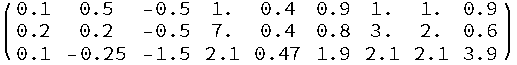
\includegraphics{refHmat.pdf}}}\intertext{with $\psi_c=\psi_\epsilon=0, \,\,  \psi_z=I$.}
  B=
\vcenter{\hbox{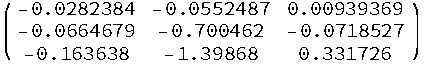
\includegraphics{refBmat.pdf}}}\\
\phi=
\vcenter{\hbox{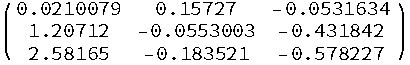
\includegraphics{refPhimat.pdf}}}\\
F=
\vcenter{\hbox{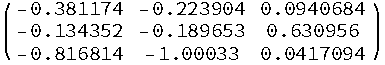
\includegraphics{refFmat.pdf}}}
\end{gather} 

}  
\end{frame}

\begin{frame}
  \frametitle{Some Time Series}


\begin{figure}
  \centering
\begin{gather}
  x_{1,t}=\alpha D_\pi(t) \\
x_{2,t}=\beta (-1)^t\\
x_{3,t}=\epsilon_t 
\end{gather} 
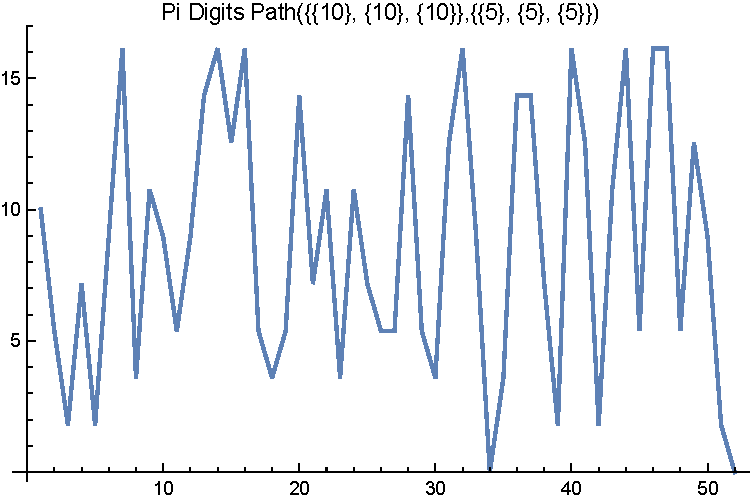
\includegraphics[width=1in]{piPath.pdf}
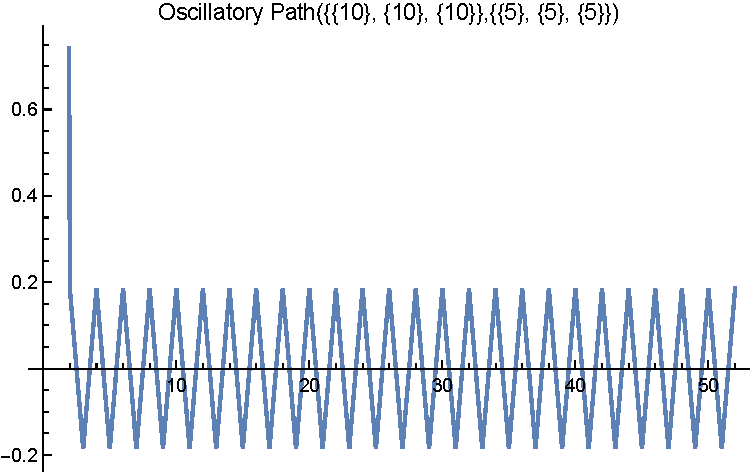
\includegraphics[width=1in]{oscillPath.pdf}
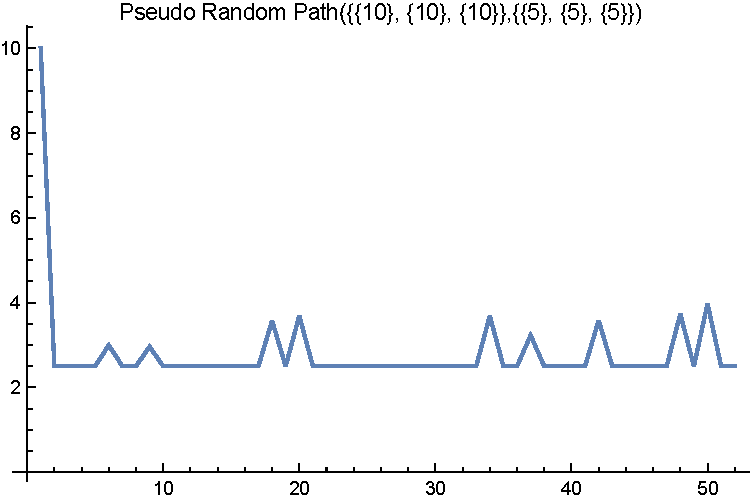
\includegraphics[width=1in]{pseudoPath.pdf}
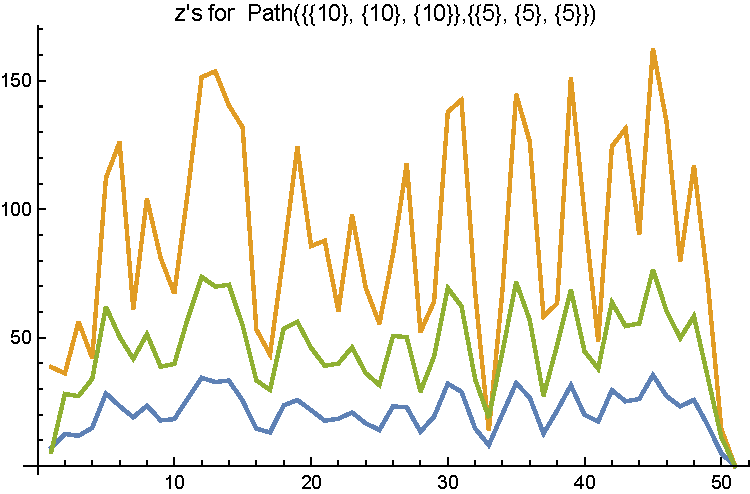
\includegraphics[width=1in]{theZs.pdf}  
  
  \caption{Arbitrary Bounded Time Series Paths and Corresponding $z_{i,t}$ values}\label{arbpaths}
\end{figure}

\begin{itemize}
\item the generated paths can depend on $x_{t-1},\epsilon_t$
  
\item apply the formula pointwise to get $z_t(x_{t-1},\epsilon_t)$
\end{itemize}

\end{frame}

\subsection{Assessing Errors}
\label{sec:assessing-errors}


\begin{frame}
  \frametitle{Truncation Error}
 	 \begin{gather}
 	 \xWOargK_t \equiv B x_{t-1}+ \phi \psi_\epsilon\epsilon  + (I - F)^{-1} \phi \psi_c + \sum_{s=0}^k F^s \phi z_{t}\label{theTruncSeries}
 \end{gather}
We can bound the  series approximation truncation errors.
Since
    \begin{gather}
      \label{eq:1}
\sum_{s=k+1}^{\infty} F^s \phi \psi_z = (I -F)^{-1} F^{k+1}\phi \psi_z       \\
\someNorm{\xWarg-\xWargK} \le\\ \someNorm{(I -F)^{-1} F^{k+1}\phi \psi_z} \left ( \someNorm{H_{-1} }+ \someNorm{H_{0} }+ \someNorm{H_{1} } \right )\bar{\mathcal{X}}
    \end{gather}

\end{frame}
\begin{frame}
  \frametitle{Truncation Error}


\begin{figure}
  \centering


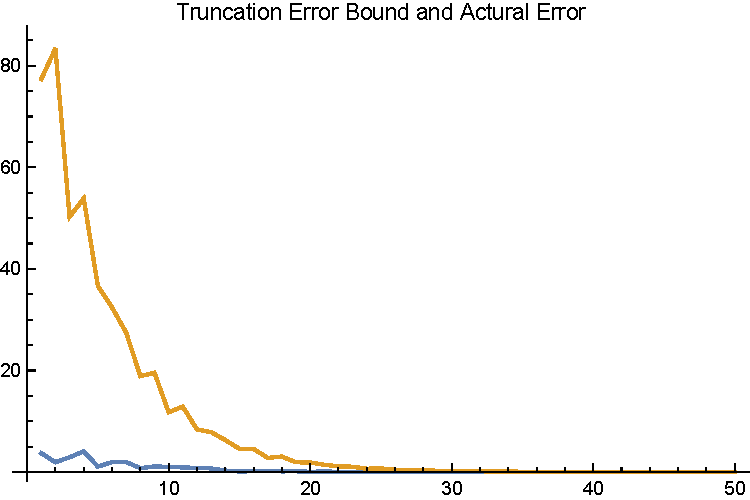
\includegraphics[width=3in]{arbTruncErr.pdf}  
  \caption{$x_t$ Error Bound Versus Actual Error} \label{figArbTrunc}

\end{figure}

\end{frame}

\begin{frame}
  \frametitle{Path Error}
One could consider approximating $\mathcal{X}_t$ using
 	 \begin{gather}
 	 \xWOargK_t \equiv B x_{t-1}+ \phi \psi_\epsilon\epsilon  + (I - F)^{-1} \phi \psi_c + \sum_{s=0}^\infty F^s \phi (z_{t}+\Delta z_{t})\label{theDeltaSeries}
 \end{gather}
We can bound the  series approximation  errors by using the largest $\Delta z_t$ in the formula. 

    \begin{gather}
\someNorm{\xWarg-\xWargK} \le \someNorm{(I -F)^{-1} \phi \psi_z}  \someNorm{\Delta z_t } \label{pathErr}
    \end{gather}

\end{frame}


\section{Nonlinear Dynamic Stochastic Time Invariant Maps}
\label{sec:extToMaps}



\subsection{Application to Time Invariant Maps}


\begin{frame}
  \frametitle{Time Invariant Maps}


  \begin{itemize}
\item  Many dynamic stochastic models 
  \begin{itemize}
  \item  have solutions that fall in this class.
\item  generate  bounded time series paths 
  \end{itemize}
  \end{itemize}



\subsection{An RBC Example}
\label{sec:rbcaux}
Consider an RBC  model described in \cite{Maliar2005}
 \begin{gather*}
   \max\left \{  u(c_t) + E_t \sum_{t=0}^\infty  \delta^{t}u(c_{t+1})\right \}\\
c_t + k_t=(1-d)k_t + \theta_t f(k_t)\\
f(k_t)= k_t^\alpha\\
u(c)=\frac{c^{1-\eta}-1}{1-\eta}
 \end{gather*}
 \end{frame}

 \begin{frame}
   \frametitle{First Order Conditions}


The well known first order conditions for the model are

\begin{tcolorbox}[ams gather]
\frac{1}{c_t^{\eta}}=\alpha \delta k_{t}^{\alpha-1} E_t \left (\frac{\theta_{t}}{c_{t+1}^\eta} \right ) \\
c_t + k_t=\theta_{t-1}k_{t-1}^\alpha \\
 \theta_t =\theta_{t-1}^\rho e^{\epsilon_t}\label{rbcSys}
 \end{tcolorbox}

\label{sec:rbcexample}

When $\eta=d=1$, we have
{\small
 \begin{gather*}
   \begin{split}
\frac{1}{c_t}=\alpha \delta k_{t}^{\alpha-1} E_t \left (\frac{\theta_{t}}{c_{t+1}} \right ) \\
c_t + k_t=\theta_{t-1}k_{t-1}^\alpha \\
\theta_t =\theta_{t-1}^\rho e^{\epsilon_t}   \end{split} \text{   leading to a closed form solution}
\begin{split}
c_t=  (1-\alpha \delta) \theta_{t} k_{t-1}^\alpha\\
  k_{t}= \alpha \delta \theta_{t} k_{t-1}^\alpha.\label{soln}\\
\theta_t =\theta_{t-1}^\rho e^{\epsilon_t}.\end{split}
\end{gather*}
}
\end{frame}

\begin{frame}

  \begin{itemize}
  \item Mean zero iid $\epsilon_t$ 
  \item compute the conditional expectation of the model variables for any given $\theta_{t-1},k_{t-1}$
\begin{gather*}
  E_t(c_t|\theta_{t-1},k_{t-1})=(1-\alpha\delta)k_{t-1}^\alpha e^{\frac{\sigma^2}{2}}\theta_{t-1}^\rho\\
  E_t(k_t|\theta_{t-1},k_{t-1})=\alpha\delta k_{t-1}^\alpha e^{\frac{\sigma^2}{2}}\theta_{t-1}^\rho\\
  E_t(\theta_t|\theta_{t-1},k_{t-1})=e^{\frac{\sigma^2}{2}}\theta_{t-1}^\rho
\end{gather*}


\item applying the law of iterated expectations
\item   compute conditional expected solution paths forward from any initial values $(x_{t-1},\epsilon_t)$.
\item use a $\linMod$ to obtain a series representation for the family of conditional expectation paths.

  \end{itemize}

\end{frame}

\begin{frame}
  
{\small

For any given values of $k_{t-1},\theta_{t-1}, \epsilon_t$ the model solution and conditional expectations path produces paths for $z_{1t}\tArg, z_{2t}\tArg, z_{3t}\tArg$

\begin{gather*}
  \begin{bmatrix}
c_t(k_{t-1},\theta_{t-1}, \epsilon_t)\\
k_t(k_{t-1},\theta_{t-1}, \epsilon_t)\\
\theta_t(k_{t-1},\theta_{t-1}, \epsilon_t)
  \end{bmatrix} \rightarrow
  \begin{bmatrix}
  z_{1t}(k_{t-1},\theta_{t-1}, \epsilon_t)\\
  z_{2t}(k_{t-1},\theta_{t-1}, \epsilon_t)\\
  z_{3t}(k_{t-1},\theta_{t-1}, \epsilon_t) 
  \end{bmatrix}\equiv z_t(k_{t-1},\theta_{t-1}, \epsilon_t)\intertext{where}
  \begin{bmatrix}
c_t(k_{t-1},\theta_{t-1}, \epsilon_t)\\
k_t(k_{t-1},\theta_{t-1}, \epsilon_t)\\
\theta_t(k_{t-1},\theta_{t-1}, \epsilon_t)
  \end{bmatrix}  =
B   \begin{bmatrix}
c_{t-1}\\
k_{t-1}\\
\theta_{t-1}
  \end{bmatrix}  + \phi \psi_\epsilon\epsilon_t + (I - F)^{-1} \phi \psi_c +\\ \sum_{\sForSum=0}^\infty F^s \phi z_{t+\sForSum}(k_{t-1},\theta_{t-1}, \epsilon_t) 
\end{gather*}
}
\end{frame}
\begin{frame}
  



For example, using the following parameter values and using the arbitrary linear reference model we can generate a series representation for the model solutions.

\begin{gather}\label{rbcparams}
\vcenter{\hbox{\includegraphics{../../paperProduction/occBind/docs/RBCParamSubs.pdf}}} \,\, \text{ we have } \,\,
  \begin{bmatrix}
    c_{ss}\\k_{ss} \\ \theta_{ss} 
  \end{bmatrix}=
\left [ \vcenter{\hbox{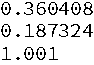
\includegraphics{RBCSSVal.pdf}}}\right ]
\end{gather}

With 
\begin{gather}\label{theInits}
  \begin{bmatrix}
 k_{t-1}\\\theta_{t-1}\\\epsilon_t 
  \end{bmatrix}=
\left [ \vcenter{\hbox{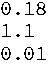
\includegraphics{anXEps.pdf}}}\right ]
\end{gather}

\end{frame}
\begin{frame}
  

\begin{figure}
  \centering
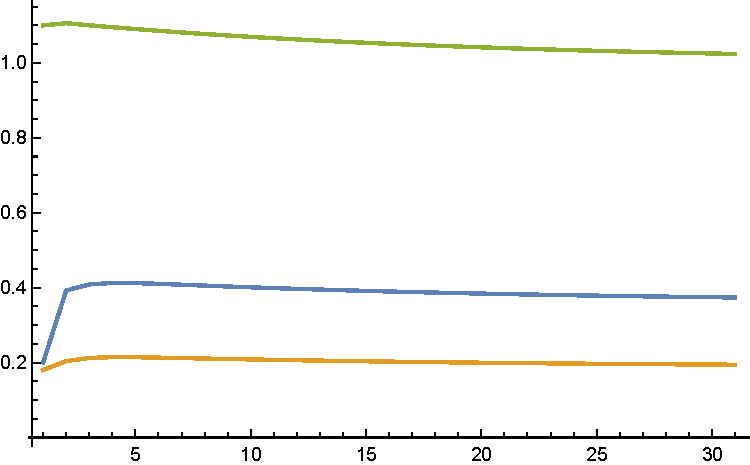
\includegraphics[width=1.7in]{simprbcvals.pdf}  
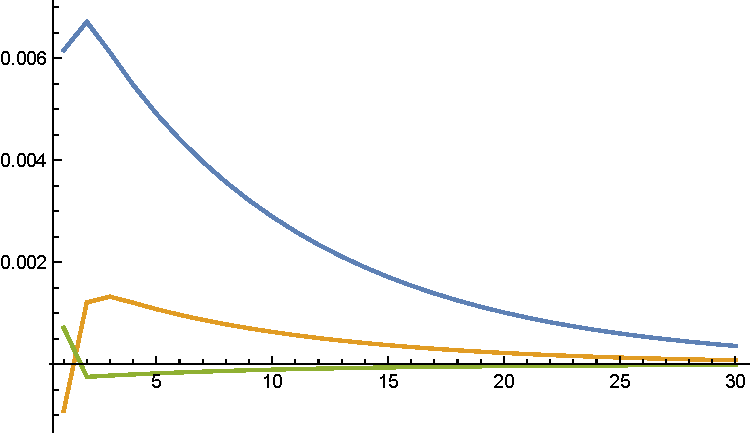
\includegraphics[width=1.7in]{simprbczvals.pdf}  
  \caption{model variable values and z values}
  \label{rbcpaths}
\end{figure}

\end{frame}

\begin{frame}
  

\begin{figure}
  \centering
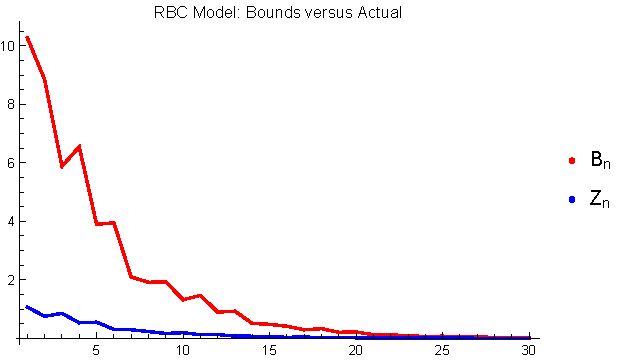
\includegraphics[width=1.7in]{simpArbBoundsVActual.pdf}  
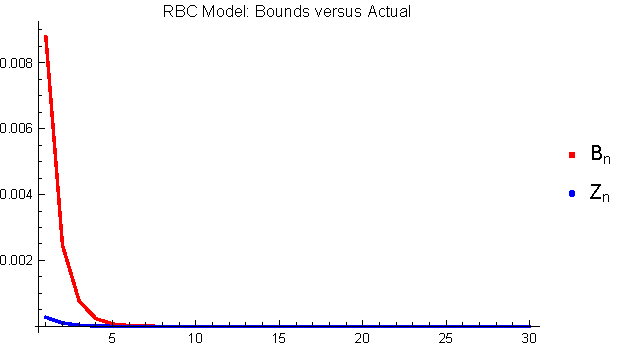
\includegraphics[width=1.7in]{simpBoundsVActual.pdf}  
  \caption{RBC Truncation Error Bound Versus Actual}
  \label{rbcTrunc}
\end{figure}
\end{frame}

\begin{frame}
  
  \begin{itemize}
  \item convenience of notation 
\begin{gather}
  h_i(x_{t-1},x_{t},x_{t+1},\epsilon_t)=h^{det}_{io}(x_{t-1},x_{t},\epsilon_t)+\\ \sum_{j=1}^{p_i} [h^{det}_{ij}(x_{t-1},x_{t},\epsilon_t)h^{nondet}_{ij}(x_{t+1})]=0
\intertext{For example, the Euler equations for the  neoclassical growth  model }
h_{10^{det}}(\cdot)=\frac{1}{c_t^\eta},\,\,
h_{11}^{det}()=\alpha \delta k_{t}^{\alpha-1} ,\,\,
h_{11}^{nondet}(\cdot)=E_t \left (\frac{\theta_{t+1}}{c_{t+1}^\eta} \right )\\
h_{20}^{det}(\cdot)=c_t + k_t-\theta_tk_{t-1}^\alpha,\,\,
h_{21}^{det}(\cdot)=0\\
h_{30}^{det}(\cdot)=\ln \theta_t -(\rho \ln \theta_{t-1} + \epsilon_t),\,\,
h_{31}^{det}(\cdot)=0
\end{gather}
  \end{itemize}

\end{frame}


\begin{frame}
  

\begin{itemize}
\item 
We now construct our linear reference model by increasing its dimension by one , $\linMod$, to accommodate 
 augmenting the RBC model with the equation
\begin{tcolorbox}[ams gather]
  \rcpC_t=\frac{\eta\theta_t}{c_t}
\end{tcolorbox}
substituting $\rcpC_{t+1}$ for $\frac{\theta_t}{c_{t+1}}$ in the first equation and 
 linearizing the RBC model about the ergodic mean
{\tiny
\begin{gather}
  \begin{bmatrix}
H_{-1}&H_{0}&H_{1} 
  \end{bmatrix}=
\vcenter{\hbox{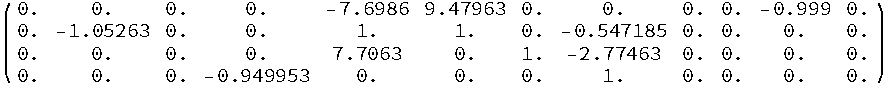
\includegraphics[width=2.4in]{RBCHmatSymb.pdf}}} \label{rbcLinSys}
\intertext{with}
\psi_\epsilon={\tiny
\begin{bmatrix}
  0\\0\\1\\0
\end{bmatrix}}, \psi_z=I
\end{gather}%(\footnote{generated by AMAPaperCalcs.mth {RBCHmatSymb.pdf}})
}
\end{itemize}
\end{frame}

 \begin{frame}
  
 \begin{itemize}
\item 

These coefficients  produce a unique stable linear solution.
{\tiny
\begin{gather}
  B=
\vcenter{\hbox{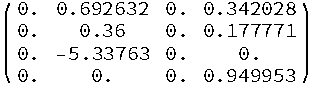
\includegraphics[width=1.7in]{RBCBmatSymb.pdf}}},
\phi=
\vcenter{\hbox{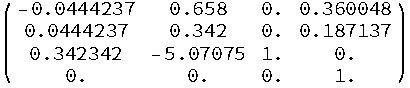
\includegraphics[width=2.2in]{RBCPhimatSymb.pdf}}}\\
F=
\vcenter{\hbox{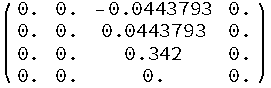
\includegraphics[width=1.7in]{RBCFmatSymb.pdf}}}
\psi_c=\vcenter{\hbox{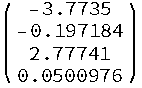
\includegraphics{RBCPsissSymb.pdf}}}
\end{gather}
}
 \end{itemize}
 \end{frame}

\section{Computing Model Solution Error Bounds}
\label{sec:solnerrorbounds}

\subsection{The Error Bound Formula Derivation}
\label{sec:errorformula}
\begin{frame}
  \frametitle{Model Definitions}
  
\begin{itemize}
\item $\eqnFuncSys$ where, each 
\begin{gather*}
\eqnFuncSysI{i}\equiv \eqnFuncSysIExpl{i} 
\end{gather*}
\item a set of model equations, $\eqnFunc_i$, 
\item  a Boolean valued gate, $\preGate_i$, $\postGate_i$,
$\lastGate_i$. 
\item exhaustive and mutually exclusive equation systems 
  \begin{itemize}
  \item complementary slackness conditions 
\item different regimes. 
  \end{itemize}
\item seeking time invariant $x_t=\xWarg$.  $\XWOarg(x_{t-1})\equiv \expct{\xWarg}$.
\end{itemize}

\end{frame}



\subsubsection{Occasionally Binding Constraints}
\label{sec:obc-solut}

\begin{frame}
  \frametitle{Occasionally Binding Constraints (OBC)}
{\tiny

Consider adding constraints 

\begin{gather*}
  I_t \ge \upsilon I_{ss}
\end{gather*}


\begin{tcolorbox}[ams gather]
if(\mu>0 \land (k_t - (1-d)k_{t-1}-\upsilon I_{ss})=0)\\
  \lambda_t -\frac{1}{c_t}\\
c_t+k_t-\theta_tk_{t-1}^\alpha\\
N_t-\lambda_t \theta_t\\
\theta_t-e^{(\rho\ln(\theta_{t-1})+\epsilon)}\\
\lambda_t + \mu_t - (\alpha k_t^{(\alpha-1)}\delta N_{t+1}+\lambda_{t+1} \delta (1-d)+\mu_{t+1}+\delta (1-d)\\
I_t-(K_t-(1-d)k_{t-1})\\
\mu_t(k_t - (1-d) k_{t-1}-\upsilon I_{ss})\\
\end{tcolorbox}
}
\end{frame}
\begin{frame}
  \frametitle{OBC Continued}
  
{\tiny
\begin{tcolorbox}[ams gather]
if(\mu=0 \land (k_t - (1-d)k_{t-1}-\upsilon I_{ss})\ge 0)\\
  \lambda_t -\frac{1}{c_t}\\
c_t+k_t-\theta_tk_{t-1}^\alpha\\
N_t-\lambda_t \theta_t\\
\theta_t-e^{(\rho\ln(\theta_{t-1})+\epsilon)}\\
\lambda_t + {\mu_t} - (\alpha k_t^{(\alpha-1)}\delta N_{t+1}+\lambda_{t+1} \delta (1-d)+{\mu_{t+1}}+\delta (1-d)\\
I_t-(K_t-(1-d)k_{t-1})\\
\mu_t(k_t - (1-d) k_{t-1}-\upsilon I_{ss})
\end{tcolorbox}
}  
\end{frame}

\subsubsection{Regime Switching}



\label{sec:regime-switch-model}

\begin{frame}
  \frametitle{Regime Switching}
  
{\tiny

Consider two states $s_t \in {0,1}$ where the depreciation rates are different:  $d_0>d_1$

\begin{gather}
    Prob(s_t=j|s_{t-1}=i)=p_{ij}
\end{gather}

For example, the Euler equations for the  neoclassical growth  model 
\label{sec:simple-rbc-model-ext} can be written as
\begin{tcolorbox}[ams gather]
if(s_t=0\land \mu>0 \land (k_t - (1-d_0)k_{t-1}-\upsilon I_{ss})=0)\\
  \lambda_t -\frac{1}{c_t}\\
c_t+k_t-\theta_tk_{t-1}^\alpha\\
N_t-\lambda_t \theta_t\\
\theta_t-e^{(\rho\ln(\theta_{t-1})+\epsilon)}\\
\lambda_t + {\mu_t} - (\alpha k_t^{(\alpha-1)}\delta N_{t+1}+\lambda_{t+1} \delta (1-d_0)+{\mu_{t+1}}+\delta (1-d_0)\\
I_t-(K_t-(1-d_0)k_{t-1})\\
\mu_t(k_t - (1-d_0) k_{t-1}-\upsilon I_{ss})\\
\end{tcolorbox}
}
\end{frame}
\begin{frame}
\frametitle{Regime Switching}
{\tiny
\begin{tcolorbox}[ams gather]
if(s_t=0\land\mu=0 \land (k_t - (1-d_0)k_{t-1}-\upsilon I_{ss})\ge 0)\\
  \lambda_t -\frac{1}{c_t}\\
c_t+k_t-\theta_tk_{t-1}^\alpha\\
N_t-\lambda_t \theta_t\\
\theta_t-e^{(\rho\ln(\theta_{t-1})+\epsilon)}\\
\lambda_t + {\mu_t} - (\alpha k_t^{(\alpha-1)}\delta N_{t+1}+\lambda_{t+1} \delta (1-d_0)+{\mu_{t+1}}+\delta (1-d_0)\\
I_t-(K_t-(1-d_0)k_{t-1})\\
\mu_t(k_t - (1-d_0) k_{t-1}-\upsilon I_{ss})
\end{tcolorbox}
}
\end{frame}
\begin{frame}
  \frametitle{Regime Switching}

{\tiny

\begin{tcolorbox}[ams gather]
if(s_t=1\land \mu>0 \land (k_t - (1-d_1)k_{t-1}-\upsilon I_{ss})=0)\\
  \lambda_t -\frac{1}{c_t}\\
c_t+k_t-\theta_tk_{t-1}^\alpha\\
N_t-\lambda_t \theta_t\\
\theta_t-e^{(\rho\ln(\theta_{t-1})+\epsilon)}\\
\lambda_t + {\mu_t} - (\alpha k_t^{(\alpha-1)}\delta N_{t+1}+\lambda_{t+1} \delta (1-d_1)+{\mu_{t+1}}+\delta (1-d_1)\\
I_t-(K_t-(1-d_1)k_{t-1})\\
\mu_t(k_t - (1-d_1) k_{t-1}-\upsilon I_{ss})\\
\end{tcolorbox}
}

\end{frame}


\begin{frame}
  \frametitle{Regime Switching}

{\tiny

\begin{tcolorbox}[ams gather]
if(s_t=1\land\mu=0 \land (k_t - (1-d_1)k_{t-1}-\upsilon I_{ss})\ge 0)\\
  \lambda_t -\frac{1}{c_t}\\
c_t+k_t-\theta_tk_{t-1}^\alpha\\
N_t-\lambda_t \theta_t\\
\theta_t-e^{(\rho\ln(\theta_{t-1})+\epsilon)}\\
\lambda_t + {\mu_t} - (\alpha k_t^{(\alpha-1)}\delta N_{t+1}+\lambda_{t+1} \delta (1-d_1)+{\mu_{t+1}}+\delta (1-d_1)\\
I_t-(K_t-(1-d_1)k_{t-1})\\
\mu_t(k_t - (1-d_1) k_{t-1}-\upsilon I_{ss})
\end{tcolorbox}
}  
\end{frame}


\begin{frame}
  \frametitle{Error Bound Formula Derivation}
  
{\small

 Given an exact solution $x^\star_t=g^\star(x_{t-1},\epsilon_t)$ define
  \begin{gather*}
G^\star(x)\equiv\expct{g^\star(x,\epsilon)} \intertext{then with}
E_tx^\star_{t+1}=G^\star(g^\star(x_{t-1},\epsilon_t))\\
    \label{eq:2}
\eqnFunc(x^\star_{t-1},x^\star_t,E_tx^\star_{t+1},\epsilon_t)=0  \,\, \forall  (x_{t-1},\epsilon_t)\\ \intertext{Using $G^\star$ and $\linMod$ construct the family of trajectories and corresponding $z^\star_t(x_{t-1},\epsilon)$ }
   x^\star_t(x_{t-1},\epsilon_t) \in{R^L}\,\,\someNorm{x^\star_t(x_{t-1},\epsilon_t)}  \le \bar{\mathcal{X}}\,\,\forall t\ > 0
  \end{gather*}
   \begin{align}
   z^\star_{t}(x_{t-1},\epsilon_t) \equiv& H_{-1}  x^\star_{t-1}(x_{t-1},\epsilon_t) + \nonumber\\
 & H_0  x^\star_{t}(x_{t-1},\epsilon_t) +  \label{defZ} \\
 & H_1  x^\star_{t+1}(x_{t-1},\epsilon_t). \nonumber
   \end{align}
}
\end{frame}

\begin{frame}
  \frametitle{Derivation Continued}
  

   The exact solution has a representation given by
	 \begin{gather}
	 x^\star_{t}(x_{t-1},\epsilon) =B x_{t-1}+ \phi \psi_\epsilon\epsilon + (I - F)^{-1} \phi \psi_c +\\ \sum_{\sForSum=0}^\infty F^s \phi z^\star_{t+\sForSum}(x_{t-1},\epsilon) \intertext{and}
	 \expct{x^\star_{t+1}(x_{t-1},\epsilon)} =B x^\star_{t+k} + \sum_{\sForSum =0}^\infty F^\sForSum \phi \expct{z^\star_{t+1+\sForSum}(x_{t-1},\epsilon)} + (I - F)^{-1} \phi \psi_c 
 \intertext{with}
 \eqnFunc(x_{t-1},x^\star_t,E_tx^\star_{t+1},\epsilon_t)=0  \,\, \forall  (x_{t-1},\epsilon_t)\\ 
	 \end{gather}
\end{frame}

\begin{frame}
  \frametitle{Derivation Continued}
  
Now consider a proposed solution for the model,
 $x^p_t=g^p(x_{t-1},\epsilon_t)$ define
$G^p(x)\equiv\expct{g^p(x,\epsilon)}$  with 
  \begin{gather}
E_tx_{t+1}=G^p(g^p(x_{t-1},\epsilon_t))\\
\eulerE_t(x_{t-1},\epsilon)\equiv
\eqnFunc(x_{t-1},x^p_t,E_tx^p_{t+1},\epsilon_t)\\\intertext{Using $G^p$ and $\linMod$ construct the family of trajectories and corresponding $z^p_t(x_{t-1},\epsilon)$ }
   x^p_t(x_{t-1},\epsilon_t) \in{R^L}\,\,\someNorm{x^p_t(x_{t-1},\epsilon_t)}  \le \bar{\mathcal{X}}\,\,\forall t\ > 0
  \end{gather}
   \begin{align}
   z^p_{t}(x_{t-1},\epsilon_t) \equiv& H_{-1}  x^p_{t-1}(x_{t-1},\epsilon_t) + \nonumber\\
 & H_0  x^p_{t}(x_{t-1},\epsilon_t) +  \label{defZ} \\
 & H_1  x^p_{t+1}(x_{t-1},\epsilon_t). \nonumber
   \end{align}


\end{frame}




\begin{frame}
  \frametitle{Derivation Continued}
  

 The proposed solution has a representation given by 
  \begin{gather}
    \label{eq:4}
	 x^p_{t}(x_{t-1},\epsilon) =B x_{t-1}+ \phi \psi_\epsilon\epsilon + (I - F)^{-1} \phi \psi_c +\\ \sum_{\sForSum=0}^\infty F^s \phi z^p_{t+\sForSum}(x_{t-1},\epsilon) 
 \intertext{and}
 	 \expct{x^p_{t+1}(x_{t-1},\epsilon)} =B x^p_{t+k} + \sum_{\sForSum =0}^\infty F^\sForSum \phi z^p_{t+1+\sForSum}(x_{t-1},\epsilon) + (I - F)^{-1} \phi \psi_c \intertext{with}
\eulerE_t(x_{t-1},\epsilon)\equiv
\eqnFunc(x_{t-1},x^p_t,E_tx^p_{t+1},\epsilon_t)
  \end{gather}

\end{frame}
  \subsection{A Conservative Bound}

\begin{frame}
  \frametitle{A Conservative Bound}
  

  \begin{gather}
    \label{eq:3}
	 x^\star_{t}(x_{t-1},\epsilon) -	 x^p_{t}(x_{t-1},\epsilon) =
\sum_{\sForSum=0}^\infty F^s \phi (z^\star_{t+\sForSum}(x_{t-1},\epsilon)-z^p_{t+\sForSum}(x_{t-1},\epsilon))     \\
	 x^\star_{t}(x_{t-1},\epsilon) -	 x^p_{t}(x_{t-1},\epsilon) =
\sum_{\sForSum=0}^\infty F^s \phi \Delta z_{t+\sForSum}(x_{t-1},\epsilon_t)   \\ 
	\someNorm{ x^\star_{t}(x_{t-1},\epsilon) -	 x^p_{t}(x_{t-1},\epsilon)} \le
\sum_{\sForSum=0}^\infty F^s \phi \someNorm{\Delta z_{t+\sForSum}(x_{t-1},\epsilon_t)}    
  \end{gather}
  \begin{itemize}
  \item $\Delta z_t$ determines accuracy
\item $\eulerE_t(x_{t-1},\epsilon)\equiv
\eqnFunc(x_{t-1},x^p_t,E_tx^p_{t+1},\epsilon_t)$ determines $\Delta z_t$ 
  \end{itemize}


\end{frame}
\begin{frame}
  \frametitle{A Conservative Bound}
  
  \begin{itemize}
  \item Assumes largest error at $t$ propagated along entire path 
  \item Easier to compute than searching along paths



  \begin{gather}
  \Delta z_t \le  \label{eq:3}
\max_{\{x_{-},\epsilon\}} \someNorm{ \phi \eqnFunc(x_{-},g^p(x_{-},\epsilon),G^p(g^p(x_{-},\epsilon)),\epsilon) }\\
	\someNorm{ x^\star_{t}(x_{t-1},\epsilon) -	 x^p_{t}(x_{t-1},\epsilon)} \le
\\ \max_{\{x_{-},\epsilon\}} \someNorm{(I-F)^{-1} \phi \eqnFunc(x_{-},g^p(x_{-},\epsilon),G^p(g^p(x_{-},\epsilon)),\epsilon) }
  \end{gather}

  \end{itemize}
\end{frame}


% \subsection{Practical Considerations for Applying the Formula}
% \label{sec:practicalformula}



 
% This section describes a method for finding maxima in a closed bounded domain.
% Let $D=[a,b]$ in $R^s$ where $a_i \le x_i \le b_i$. We want to find  $M=f(x^\ast)= \max_{x \in D}f(x)$.
% Th number theoretic (Quasi-Monte Carlo) approached is designed for finding optima with many local optima.  It is based on the used of space filling points.\cite{Xu2005}
% The number theoretic method of optimization includes two basic steps.
% \begin{enumerate}
% \item Choose a set $p=x_i, i=1,\dots,n$ of potential optima that are uniformly scattered.
% \item Find $M_n\text{ and } x^\ast \in p =\max_{1\le i \le n}f(x_i)$
% \end{enumerate}

% Even when choosing $p$ wisely convergence slow until \cite{Niederreiter1983}.  They speed up the convergence by contracting the domain.
% Their algorithm discards all but the best in the domain. Must have very many points to guarantee choosing a point close to the optimum.


% MSNTO selects a finite number of sample points uniformly scattered on D.  Next it discard inferior points retaining small sample of potential maxima.  These form the clusters for the next step.  The algorithm performs a domain contraction on each of the clusters.






\section{Improving Proposed  Solutions}
\label{sec:algoforsoln}

\subsection{Algorithm Overview}
\label{sec:pseudocode}
\begin{frame}
  \frametitle{Algorithm Overview}
{\small
  \begin{itemize}
  \item Consider the single model case $  \eqnFunc(x_{t-1},x_t,\expct{x_{t+1}},\epsilon)=0$.  
\item We seek $\eqnFunc(x_{t-1},\xWOarg^\star\tArg,\XWOarg^\star(\xWOarg^\star\tArg),\epsilon)=0\,\,\forall \tArg $
\item Given a proposed model solution $x_t=\xWOarg^p\tArg$ compute $\XWOarg^p(x_{t-1})\equiv \expct{\xWOarg^p\tArg}$. 
\item we will use a linear reference model $\linMod  \equiv \linModMats$ 
to construct a series of $\zpWOarg$ functions that improve the accuracy of the proposed solution.
\end{itemize}<
}
\end{frame}
\begin{frame}
  \frametitle{Constructing the $\zWOarg$ Series}

\begin{gather*}
 \intertext{We can define functions $\zpWOarg,\ZpWOarg$ by}
\zpWarg\equiv H
\begin{bmatrix}
x_{t-1}\\ \xpWarg\\ \XpWOarg(\xWarg)
\end{bmatrix}+\phi_\epsilon \epsilon_t+\phi_c\\
\ZpWOarg(x_{t-1})\equiv \expct{\zpWarg}
\end{gather*}
 \begin{itemize}
\item  define conditional expectations paths for $x_t, z_t$ -- {\color{green} Algorithm loop begins here.}
 \begin{gather*}
 x_{t+k+1}=\XpWOarg(x_{t+k}),\,\,\,z_{t+k+1}=\ZpWOarg(x_{t+k})\,\,\,\,  \forall k\ge 0      \end{gather*}
% \item
% it will be useful to construct an augmented decision rule,
% $\ADR\tArg\equiv
%   \begin{bmatrix}
%     x^p\tArg\\z^p\tArg
%   \end{bmatrix}$, initially $z^p\tArg=0$
   \end{itemize}

\end{frame}
\begin{frame}
  \frametitle{Using the $\zpWarg$ Series}
{\small
  \begin{itemize}
  \item We get expressions for $x_t, \expct x_{t+1}$ consistent with $\linMod$ and the conditional expectations path
   \begin{gather*}
     \mathcal{X}_{t} =B x_{t-1}+ \phi \psi_\epsilon\epsilon + (I - F)^{-1} \phi \psi_c + \sum_{\sForSum=0}^\infty F^s \phi \ZpWOarg(x_{t+\nu})\\
	\expct{ \mathcal{X}_{t+1}} =B \mathcal{X}_{t}  + (I - F)^{-1} \phi \psi_c+ \sum_{\sForSum =0}^\infty F^{\sForSum-1} \phi \ZpWOarg(x_{t+\nu}) \,\,\,\,\,\forall t,k \ge  0
\end{gather*}
\item Use the model equations, $\eqnFuncSys$ and $x_t\tArg=\mathcal{X}_t\tArg$ to determine $\xppWarg, \zppWarg$
\item $\xpWarg=\xppWarg, \zpWarg=\zppWarg$ -- {\color{green} Repeat loop.}
  \end{itemize}
}
\end{frame}

%% \begin{frame}
%%   \includegraphics[width=2in]{resDir/forBetterRBC--1,1,1-Iters30theK0host-MacBook-Pro-2numKern2Trad.pdf}  
%%   \includegraphics[width=2in]{resDir/forBetterRBC--1,1,1-Iters30theK0host-MacBook-Pro-2numKern2ApproxTrad.pdf}
%% \end{frame}

%% \begin{frame}
%%     \includegraphics[width=2in]{resDir/forBetterRBC--1,1,1-Iters30theK0host-MacBook-Pro-2numKern2Approx.pdf}
%%   \includegraphics[width=2in]{resDir/forBetterRBC--1,1,1-Iters30theK0host-MacBook-Pro-2numKern2.pdf}

%% \end{frame}
%% \begin{frame}
%%   \includegraphics[width=2in]{resDir/forBetterRBC--1,1,1-Iters30theK30host-MacBook-Pro-2numKern2Approx.pdf}
%%   \includegraphics[width=2in]{resDir/forBetterRBC--1,1,1-Iters30theK30host-MacBook-Pro-2numKern2.pdf}

%% \end{frame}

%% \begin{frame}
%%     \includegraphics[width=2in]{resDir/forBetterRBC--3,3,3-Iters20theK20numKern2.pdf}

%% \end{frame}
\subsection{{Some Algorithmic Details}}


\begin{frame}
  \frametitle{Some Algorithmic Details}
  


\begin{enumerate}
\item Not required, but one can use a linearized version of some $\eqnFunc_i$  as the  linear reference model, $\linMod$.
\item Current implementation builds on the approach described in \cite{Judd2014}
  \begin{itemize}
  \item Approximate the ``boundaries'' for the ergodic set
  \item Decide upon the degrees of approximation for the an-isotropic Smolyak polynomial representation
  \item Precalculate all integrals
  \end{itemize}
\item Uses the $\linMod$ linear decision rule as an initial guess for decision rule $\xpWarg$ to obtain conditional expectations function
\item Linearities in series expressions exploited
\item Highly parallelizable 
\end{enumerate}


\end{frame}







\section{Conclusions}
\label{sec:conclusions}


\begin{frame}
  \frametitle{Next Steps}
\begin{itemize}
\item Exploit parallelism
\item Support Vector Machine Regression (SVMR)
\item Large Model Implementation
\item Improve Error Bounds
%\item Application to \cite{feng14:_num}
\item Dynare Interface
\end{itemize}

\end{frame}



\bibliographystyle{plainnat}
\bibliography{anderson,files}

\end{document}
